\documentclass[t]{beamer}
\usepackage[english]{babel}
\usepackage[utf8]{inputenc}
\usepackage[T1]{fontenc}
\usepackage{amsmath}
\usepackage{amssymb}
\usepackage{amsfonts}
\usepackage{amsthm}
\usepackage{graphicx}
\usepackage{xcolor}
\usepackage[scaled]{helvet}
\renewcommand{\familydefault}{\sfdefault}

\usepackage{bm}
\usepackage{subcaption}
\usepackage{xcolor}
\usepackage{soul}
\usepackage{enumitem}
\usepackage{tikz}

\usepackage[backend=biber,style=abnt,maxbibnames=3,maxcitenames=1,uniquelist=false, uniquename=full,doi,url=false]{biblatex}
\renewcommand*{\bibfont}{\scriptsizsmalle}

\AtEveryBibitem{% Clean up the bibtex rather than editing it
    \clearlist{address}
    \clearfield{date}
    \clearfield{eprint}
    \clearfield{isbn}
    \clearfield{issn}
    \clearlist{location}
    \clearfield{month}
    \clearfield{series}

    \ifentrytype{book}{}{% Remove publisher and editor except for books
	\clearlist{publisher}
	\clearname{editor}
    }
}

\usefonttheme[onlymath]{serif}
\addbibresource{../aftertext/references.bib} % Seus arquivos de referências

\newcommand{\R}{\mathbb{R}} 
\newcommand{\N}{\mathbb{N}} 

\newcommand{\highlight}[1]{%
  \colorbox{yellow!50}{$\displaystyle#1$}}

\renewcommand*\footnoterule{}

\definecolor{tabblue}{RGB}{0,107,164}
\definecolor{taborange}{RGB}{255,128,14}
\definecolor{tabgray}{RGB}{171,171,171}
\definecolor{tabdarkgray}{RGB}{89,89,89}

%%%
%%% Define cores
%%%
\definecolor{cinza}{HTML}{75818B}

%%%
%%% Remove a barra de navegação do Beamer
%%%
\setbeamertemplate{navigation symbols}{}

%%%
%%% Margem dos slides
%%%
\setbeamersize{text margin left=10mm,text margin right=5mm} 

%%%
%%% Redefine a fonte do título dos slides
%%%
\setbeamercolor{frametitle}{fg=cinza}
\setbeamerfont{frametitle}{series=\bfseries}
\setbeamerfont{frametitle}{size=\huge}

%%%
%%% Ajusta a posição do título dos slides e início do texto
%%%
\addtobeamertemplate{frametitle}{\vspace*{2mm}}{\vspace*{5mm}}

%%%
%%% Adiciona páginação nos slides
%%%
%%% Caso não queira, basta comentar este bloco inteiro
%%% para ocultar a paginação
%%%
\addtobeamertemplate{navigation symbols}{}{
\usebeamerfont{footline}
\usebeamercolor[fg]{footline}
}
\setbeamercolor{footline}{fg=cinza}
\setbeamerfont{footline}{series=\bfseries}
\setbeamerfont{footline}{size=\tiny}
\setbeamertemplate{footline}{
\usebeamerfont{page number in head}
\usebeamercolor[fg]{page number in head}
\hspace{5mm}
\insertframenumber/\inserttotalframenumber
\vspace{5mm}
}

%%%
%%% Redefine símbolo padrão do itemize
%%%
\setbeamertemplate{itemize items}[ball]

%%%
%%% Insere numeração nas figuras
%%%
\setbeamertemplate{caption}[numbered]

%%%
%%% Imagem de fundo a ser usada em todos os slides (exceto
%%% no primeiro e no último)
%%%
\usebackgroundtemplate
{

\includegraphics[width=\paperwidth,height=\paperheight]{fundo.png}
}

%%%
%%% Adiciona slide de "Estrutura"
%%%
\AtBeginSection[]{\frame{\frametitle{Agenda}\tableofcontents
[current]}}

%%%
%%% Define fontes e cores do slide de "Estrutura"
%%%
\setbeamerfont{section in toc}{series=\bfseries}
\setbeamercolor{section in toc}{fg=gray}
\setbeamerfont{section in toc shaded}{series=\mdseries}
\setbeamercolor{section in toc shaded}{fg=gray!01}
\setbeamercolor{subsection in toc}{fg=cinza}
\setbeamercolor{subsection in toc shaded}{fg=gray!60}
\setbeamercolor{subsubsection in toc}{fg=cinza}
\setbeamercolor{subsubsection in toc shaded}{fg=gray!60}

\mode<presentation>
%%%
%%% Início
%%%
\begin{document}

%%%
%%% Slide da capa
%%%
{
\usebackgroundtemplate{
\includegraphics[width=\paperwidth]{capa.png}}
\begin{frame}[plain,noframenumbering]
\vspace{18mm}
%%%
%%% Título da Apresentação
%%%
\begin{flushright}
\textcolor{cinza}{\textbf{\Large{
Physics-Informed DEQs for Solving ODEs
}}}
\end{flushright}

\vspace{-6mm}
%%%
%%% Nome do autor
%%%
\begin{flushright}
\textcolor{cinza}{\textbf{\scriptsize{
Bruno M. Pacheco
}}}
\end{flushright}

\vspace{-7mm}
%%%
%%% Formação | Departamento | Centro
%%%
\begin{flushright}
\textcolor{cinza}{\scriptsize{
Projeto de Fim de Curso | DAS
}}
\end{flushright}


\end{frame}
}

%%%
%%% Motivação
%%%

\begin{frame}
    %\frametitle{Motivation}
    \begin{columns}
        \begin{column}{0.5\textwidth}
	    \begin{itemize}[label={\textbullet}]
	        \item Good results on previous works with PINNs
		\item Interest from the Learning \& Dynamical Systems community on implicit models
	    \end{itemize}
	    \begin{figure}[h]
	        \centering
	        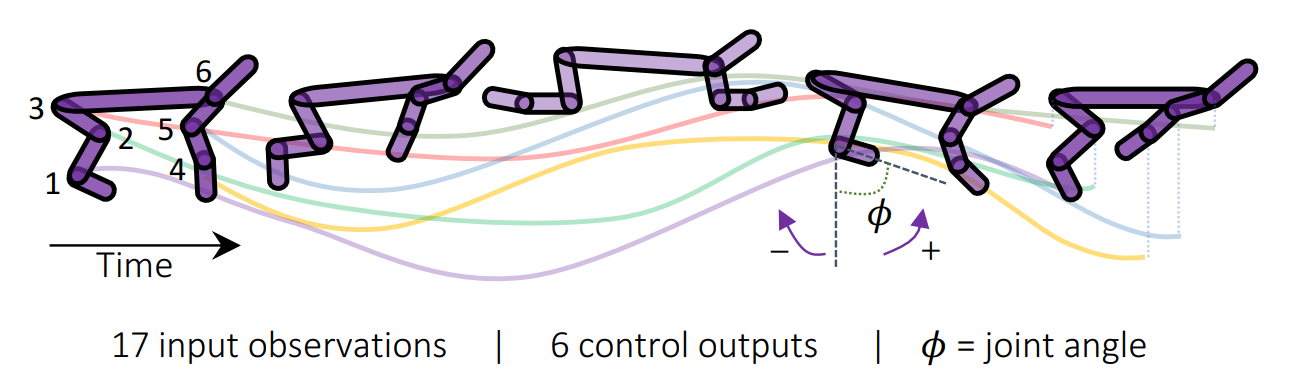
\includegraphics[width=0.8\textwidth]{ltc.png}
		\cite{Ramin_ltc_2020}
	    \end{figure}
        \end{column}
	\begin{column}{0.5\textwidth}
	    \begin{figure}[h]
	        \centering
	        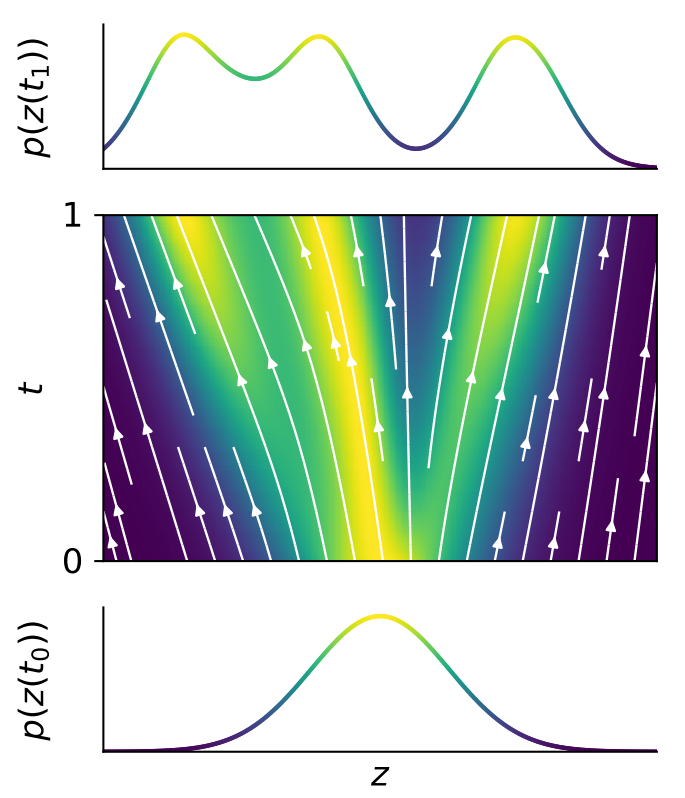
\includegraphics[width=0.6\textwidth]{normalizing-flows.png}
		\cite{Gratwohl_ffjord_2018}
	    \end{figure}
	\end{column}
    \end{columns}
    \quad

    \quad

	    "Implicit layers [models] refer to techniques where the forward pass of a network is computed via non-linear dynamical systems, such as fixed-point or differential equation solutions, with the backward pass computed via the implicit function theorem." \cite{NEURIPS2021_4ffbd5c8}
\end{frame}

%%%
%%% Objetivo do PFC
%%%

% \begin{frame}
% \frametitle{Goal}
% \textbf{Study}, \textbf{implement} and \textbf{validate} the use of \emph{Deep Equilibrium models} (DEQs) as effective and efficient solvers for initial value problems (IVPs), making use of \emph{physics-informed} training.
% 
% \begin{itemize}
%     \item<2-> \textbf{Study} PINNs and DEQs;
%     \item<3-> \textbf{Implement} a PIDEQ;
%     \item<4-> \textbf{Validate} PIDEQ as an IVP solver.
% \end{itemize}
% \end{frame}


%%%
%%% Demais slides (exceto o slide final)
%%%
\begin{frame}
\frametitle{Agenda}
\tableofcontents
\end{frame}

\section{Background}

\subsection{Partial Differential Equations}

\begin{frame}
    \frametitle{Partial Differential Equations (PDEs)}
    PDEs usually describe the relationship between unknown quantities and their rates of change in time and space.
    \begin{equation}
	\frac{d \bm{y}\left( \bm{x}, t \right) }{d t} = \mathcal{N}\left( t, \bm{x}, \bm{y}\left( \bm{x},t \right)  \right) 
    \end{equation}\pause

    \emph{Boundary Value Problems} (BVPs):
    \begin{align*}
	\phi :\R^{n+1}&\to \R^{m} &\\
	\text{s.t.} \quad \frac{d \phi\left( \bm{x},t \right) }{d t} &= \mathcal{N}\left( \bm{x},t, \phi\left( \bm{x},t \right)  \right), \quad t\in I, \bm{x}\in X \\
	\alpha_i\phi\left( \bm{x},t \right) + \beta_i \frac{d \phi\left( \bm{x},t \right) }{d t} &= \bm{f}_i\left( \bm{x},t \right), \quad\quad\bm{x}\in X_0^{(i)}, t\in I_0^{(i)}, i=1,\ldots
    \end{align*}
\end{frame}

\begin{frame}
    \frametitle{Van der Pol oscillator (VdP)}
    Widely used ODE to model natural phenomena \[
    \frac{d}{dt}\begin{bmatrix} y_1\left( t \right) \\ y_2\left( t \right)  \end{bmatrix} = \begin{bmatrix} 
y_2\left( t \right) \\
\mu\left( 1-y_1\left( t \right) ^2 \right) y_2\left( t \right) - y_1(t)
\end{bmatrix} 
    ,\] where $\mu$ controls the dampening of the oscillation.

    \pause
    \quad

    VdP has no analytical solution \cite{panayotounakos_lack_2003}, so it is widely used as a benchmark.
    % \footnotetext{\tiny PANAYOTOUNAKOS, D.e.; PANAYOTOUNAKOU, N.d.; VAKAKIS, A.f. 2003. On the lack of analytic solutions of the Van der Pol oscillator.}
\end{frame}

\begin{frame}
    \begin{figure}[h]
	\centering
	\begin{subfigure}[b]{\textwidth}
	    \centering
	    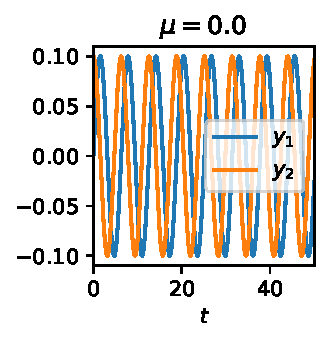
\includegraphics[width=0.3\textwidth]{../images/vdp_timeplot_mu_00.pdf}
	    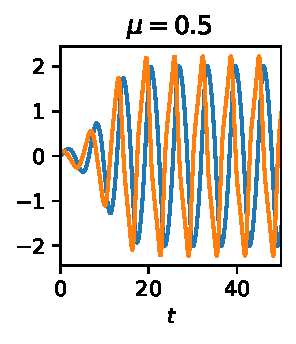
\includegraphics[width=0.27\textwidth]{../images/vdp_timeplot_mu_05.pdf}
	    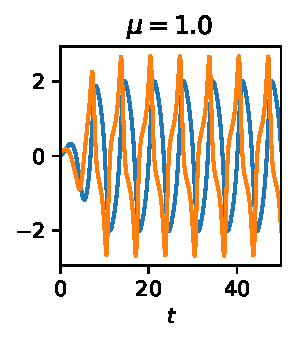
\includegraphics[width=0.27\textwidth]{../images/vdp_timeplot_mu_10.pdf}
	    %\caption{Time evolution}\label{fig:vdp_timeplots}
	\end{subfigure}
	\begin{subfigure}[b]{\textwidth}
	    \centering
	    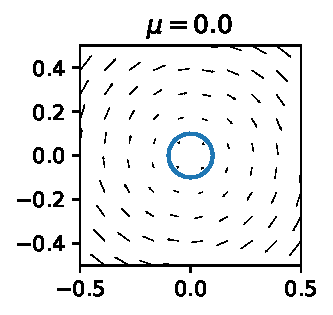
\includegraphics[width=0.3\textwidth]{../images/vdp_statespace_mu_00.pdf}
	    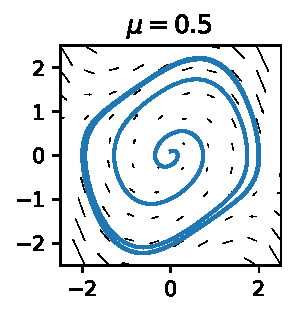
\includegraphics[width=0.27\textwidth]{../images/vdp_statespace_mu_05.pdf}
	    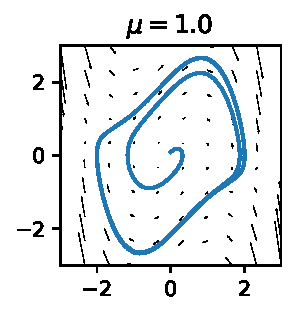
\includegraphics[width=0.27\textwidth]{../images/vdp_statespace_mu_10.pdf}
	    %\caption{State-space}\label{fig:vdp_statespace}
	\end{subfigure}
	\caption{Examples of (numerical) solutions to the Van der Pol oscillator with different dampening behavior for $\phi(0)=\bm{0}$.}\label{fig:vdp_example}
    \end{figure}
\end{frame}

\begin{frame}
    \frametitle{Nonlinear Schrödinger (NLS)}
    Nonlinear version of the classical Schrödinger equations, applies to the propagation of light in nonlinear optical fibers and others.  \[
    \frac{d y}{dt}\left( x,t \right)  = i\frac{1}{2}\frac{\partial^2 y}{\partial x^2} + i|y|^2y
    \]

    \pause
    \quad

    In the NLS, $y$ is a complex function, but it is usually modeled as a function on $\R^2$.
\end{frame}

\begin{frame}
    \vfill
    \begin{figure}[h]
        \centering
        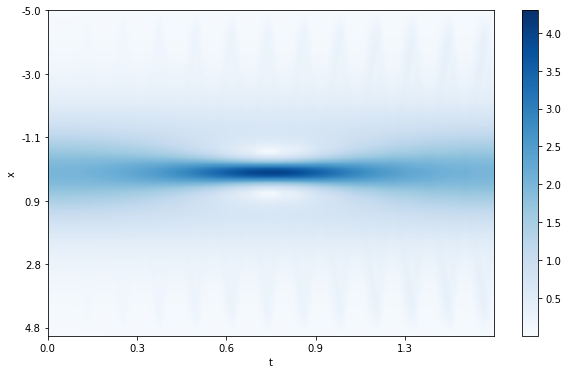
\includegraphics[width=0.8\textwidth]{nls.png}
        \caption{Example solution to the NLS on a periodic domain.}
        \label{fig:nls-example}
    \end{figure}
\end{frame}

\subsection{Physics-Informed Neural Networks}

\begin{frame}
    \frametitle{Physics-Informed Neural Networks}
    Let us define a neural network as a function
    \begin{align*}
	D^{FN}_{\bm{\theta}}: \R^{n+1} &\longrightarrow \R^{m} \\
	\bm{x},t &\longmapsto 	D^{FN}_{\bm{\theta}}(\bm{x}, t) = \bm{z}^{[L]}
    \end{align*}
    with $L$ layers such that
    \begin{align*}
	\bm{z}^{[0]} &= \left( \bm{x},t \right)  \\
	\bm{z}^{[i]} &= f^{[i]}_{\bm{\theta}}\left( \bm{z}^{[i-1]} \right) ,\,i=1,\ldots,L
    .\end{align*}
\end{frame}

\begin{frame}
    \frametitle{Physics-Informed Neural Networks}

    \begin{figure}[h]
        \centering
        \includegraphics[width=0.8\textwidth]{deep-feedforward-network.pdf}
        \caption{Deep Feedforward Network.}
        \label{fig:deep-feedforward-network-pdf}
    \end{figure}
\end{frame}

\begin{frame}
    \frametitle{Physics-Informed Neural Networks}
    Traditionally, training such neural network to solve a PDE would require to optimize \[
	\min \sum_{\bm{x}\in X, t\in I} \|D^{FN}_{\bm{\theta}}(\bm{x}, t) - \phi(\bm{x}, t)\|
    ,\] 
    which would be senseless! \pause

    A PINN\cite{Raissi2019}, on the other hand, is trained on \[
    \min \sum_{\bm{x}\in X, t \in I} \left\|  \frac{d D^{FN}_{\bm{\theta}}(\bm{x}, t)}{dt} - \mathcal{N}\left( \bm{x}, t, D^{FN}_{\bm{\theta}}(t) \right) \right\| 
    ,\] 
    optimizing the \emph{dynamics} of the network.
\end{frame}

\begin{frame}
    \frametitle{Physics-Informed Neural Networks}
    More precisely, the training is on \[
	\min_{\bm{\theta}} J_b\left( \bm{\theta} \right) + \lambda J_{\mathcal{N}}\left( \bm{\theta} \right)
    ,\] with
    \begin{align*}
	J_b\left( \bm{\theta} \right) &= \sum_{\bm{x}_0,t_0,i} \|\alpha_iD^{FN}_{\bm{\theta}}\left( \bm{x}_0,t_0 \right) + \beta_i \frac{d D^{FN}_{\bm{\theta}}\left( \bm{x}_0,t_0 \right) }{d t} - \bm{f}_i\left( \bm{x}_0,t_0 \right)\| \\
	J_{\mathcal{N}}\left( \bm{\theta} \right) &= \sum_{t \in I_{\mathcal{N}},\bm{x}\in X_{\mathcal{N}}} \left\| \frac{d D^{FN}_{\bm{\theta}}\left( \bm{x}, t \right) }{dt} - \mathcal{N}\left( \bm{x}, t,D^{FN}_{\bm{\theta}}\left( \bm{x}, t \right)  \right)  \right\|
    ,\end{align*}
    in which $I_{\mathcal{N}}\subset I$ and $X_{\mathcal{N}}\subset X$ are sets of random points from the domain.
\end{frame}

\begin{frame}
    \begin{figure}[h]
        \centering
        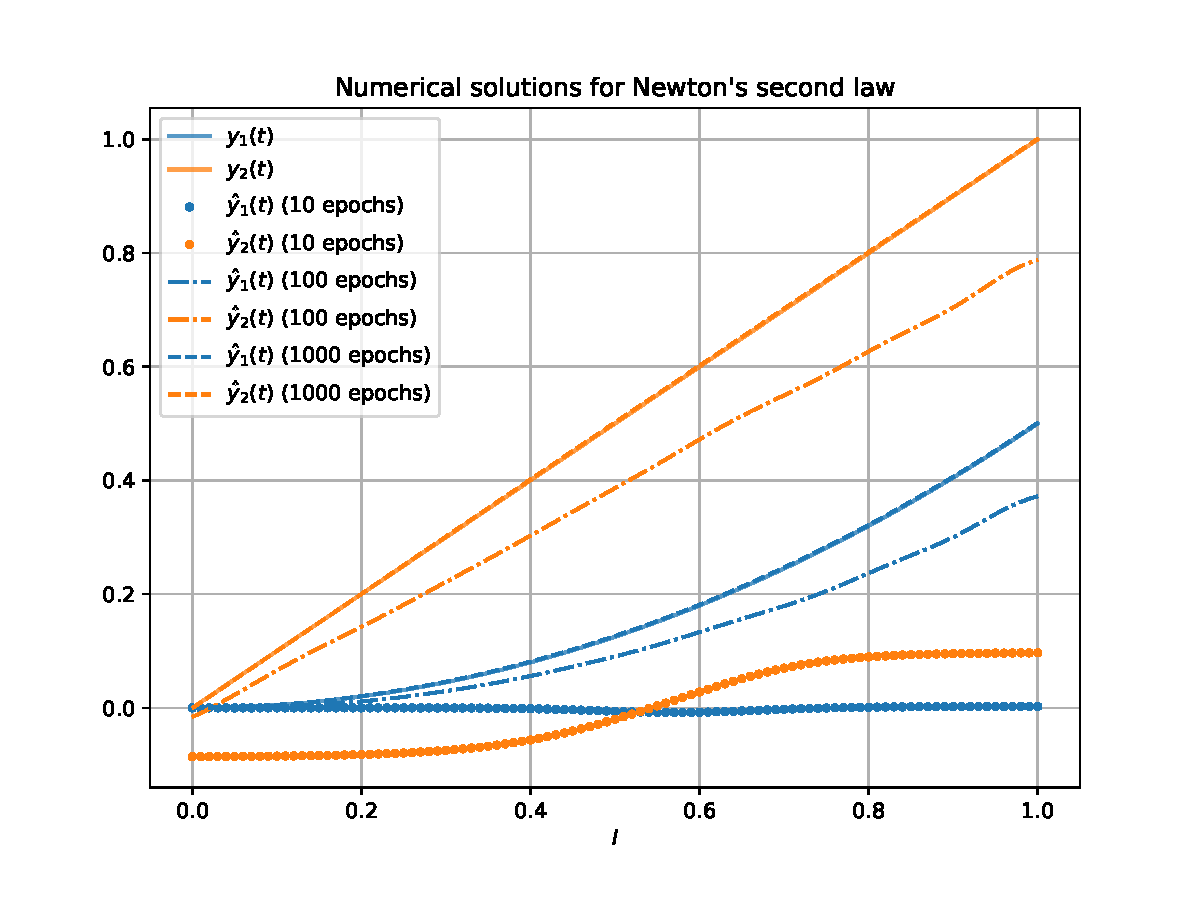
\includegraphics[width=0.8\textwidth]{../images/pinn_newton.pdf}
        \caption{Example of PINN trained to solve IVP of Newton's second law with $y(0)=0$ and constant force. $y_1$ is the velocity and $y_2$ is the acceleration.}
        \label{fig:-images-pinn_newton-pdf}
    \end{figure}
\end{frame}

\subsection{Deep Equilibrium Models}

\begin{frame}
    \frametitle{Deep Equilibrium Models}
    \begin{columns}
	\column{0.5\textwidth}
	Deep Feedforward Network:
	\begin{align*}
	    D^{FN}_{\bm{\theta}}: \R^{n+1} &\longrightarrow \R^{m} \\
	    \bm{x}, t &\longmapsto D^{FN}_{\bm{\theta}}(\bm{x},t) = \bm{z}^{[L]} \\
	    z^{[0]} =&\, (\bm{x}, t) \\
	    \bm{z}^{[i]} =&\, f^{\highlight{[i]}}_{\bm{\theta}}\left( \bm{z}^{[i-1]} \right) , i\highlight{=1,\ldots,L}
	\end{align*} \pause
	\column{0.5\textwidth}
	Deep Equilibrium \hl{Model}:
	\begin{align*}
	    D^{EQ}_{\bm{\theta}}: \R^{n+1} &\longrightarrow \R^{m} \\
	    \bm{x}, t &\longmapsto D^{EQ}_{\bm{\theta}}(\bm{x},t) = \bm{z}^{[\infty]} \\
	    z^{[0]} =&\, (\bm{x}, t) \\
	    \bm{z}^{[i]} =&\, f_{\bm{\theta}}\left( \bm{z}^{[i-1]} \right) , i\highlight{\to \infty}
	\end{align*}
    \end{columns}
\end{frame}

\begin{frame}
    \frametitle{Deep Equilibrium Models}
    $\bm{z}^{[\infty]}$ exists (and is well-defined) iff $\left\{  \bm{z}^{[i]} \right\}$ converges.
    \linebreak

    Then, $\exists N\in \N$ such that $\forall i\ge N,\,z^{[i]}\approx z^{[i+1]}$.
    \linebreak

    Therefore, $\bm{z}^{\star}=\bm{z}^{[\infty]}\approx \bm{z}^{[N]}$,
    \linebreak

    and $\bm{z}^{\star}$ is an \emph{equilibrium point} of $f_{\bm{\theta}}$ \[
	    \bm{z}^{\star} = f_{\bm{\theta}}\left( \bm{z}^{\star} \right)
    .\] 
\end{frame}

\begin{frame}
    \frametitle{Deep Equilibrium Models}
    Definition \cite{Bai2019}:
    \begin{align*}
	D^{EQ}_{\bm{\theta}}: \R^{n+1} &\longrightarrow \R^{m} \\
	\bm{x},t &\longmapsto 	D^{EQ}_{\bm{\theta}}(\bm{x},t) = \bm{z}^{\star} \\
	\bm{z}^{\star} &= f_{\bm{\theta}}\left( \bm{x},t, \bm{z}^{\star} \right)
    .\end{align*}

    \pause
    \begin{figure}[h]
        \centering
        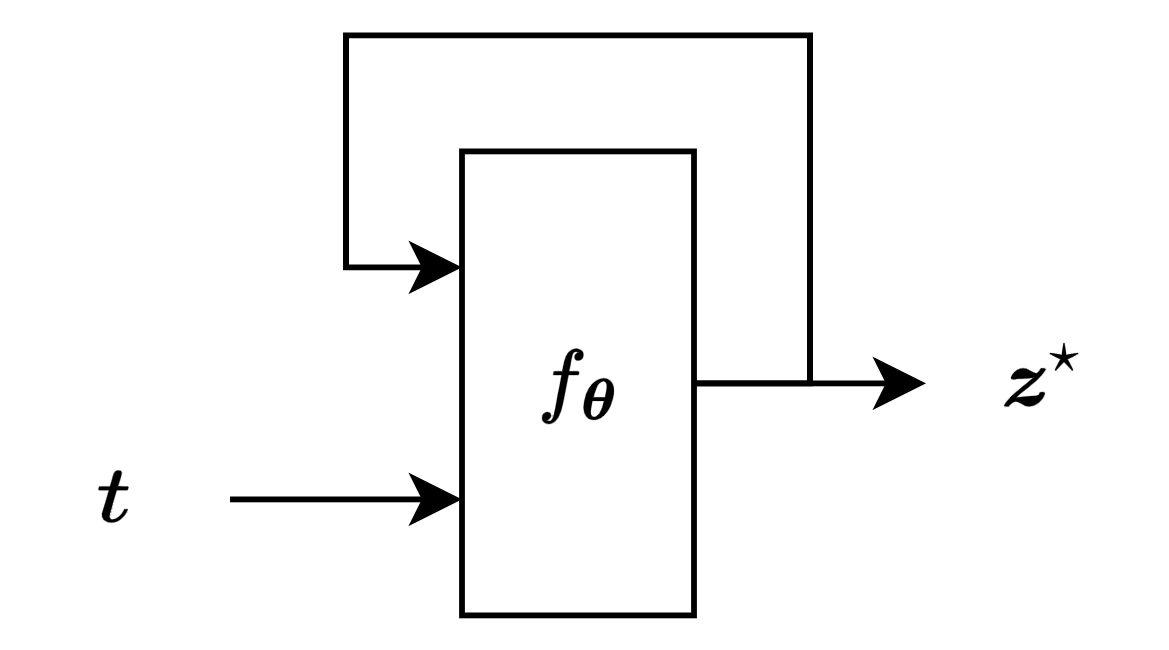
\includegraphics[width=0.5\textwidth]{deq-diagram.pdf}
        \caption{DEQ diagram.}
        \label{fig:deq-diagram-}
    \end{figure}
\end{frame}

\begin{frame}
    \frametitle{DEQ Capacity}
    \vfill
    Restricting every layer of the networks to be the same is not an actual restriction, as a DEQ can model a large number of deep neural networks, including CNNs, RNNs, ResNets, and many others.
    \vfill
\end{frame}

\begin{frame}
    \frametitle{DEQ Capacity}

    E.g., given a deep feedforward network \[
	\bm{z}^{[i+1]} = \sigma^{i}\left( W^{[i]}\bm{z}^{[i]} + \bm{b}^{[i]} \right),\,i=0,\ldots,L-1,\,\bm{z}^{[0]} = \bm{u}
    ,\]
    it is not hard to see that it is equivalent to a DEQ with \[
	\bm{z} = \sigma\left( W_z\bm{z} + W_u\bm{u} + \bm{\tilde{b}} \right) 
    \] where \[
    W_z=\begin{bmatrix} 
	0 & \hdots & 0 & 0 \\
	W^{[1]} & \hdots & 0 & 0 \\
	\vdots & \ddots & \vdots & \vdots \\
	0 & \hdots & W^{[L-1]} & 0
    \end{bmatrix},
    W_x = \begin{bmatrix} W^{[0]} \\ 0 \\ \vdots \\ 0 \end{bmatrix} ,
    \bm{\tilde{b}} = \begin{bmatrix} \bm{b}^{[0]} \\ \vdots \\ \bm{b}^{[L-1]} \end{bmatrix}
    .\] 
\end{frame}

\begin{frame}
    \frametitle{Forward Pass}
    $\bm{z}^{\star}$ is an equilibrium of $f_{\bm{\theta}} \iff \bm{z}^{\star}$ is a root of $g_{\bm{x},t}(\bm{z}) = f_{\bm{\theta}}(\bm{x},t,\bm{z}) - \bm{z}$.
    \linebreak

    Therefore, \[
	D^{EQ}_{\bm{\theta}}(\bm{x},t) = \bm{z}^{\star} = RootFind(g_{\bm{x},t})
    ,\] in which $RootFind$ is any root-finding algorithm (e.g., simple iteration, Newton's method, quasi-Newton methods).
\end{frame}

\begin{frame}
    \frametitle{Backward Pass}
    By the definition of the model's output, \[
	g_{\bm{x},t}(D^{EQ}_{\bm{\theta}}(t)) = 0
    ,\] i.e., $D^{EQ}_{\bm{\theta}}$ is a \emph{parametrization} of $z$ with respect to $t$ for $g_{\bm{x},t}(\bm{z})=0$.
    \linebreak

    Consequently, by the implicit function theorem \cite{Bai2019}, \[
	\frac{d g_{\bm{x},t}}{d \bm{\theta}}(D^{EQ}_{\bm{\theta}}(\bm{x},t)) = \frac{d g_{\bm{x},t}}{d \bm{z}}(D^{EQ}_{\bm{\theta}}(\bm{x},t)) \frac{d D^{EQ}_{\bm{\theta}}}{d \bm{\theta}}(\bm{x},t)
    .\] 
\end{frame}

\begin{frame}
    \frametitle{Backward Pass}
    
    By the definition of $g_{\bm{x},t}$ we know that \[
	\frac{d g_{\bm{x},t}}{d \bm{z}}(\bm{z}) = \frac{d f_{\bm{\theta}}}{d \bm{z}}(\bm{x},t,\bm{z}) - I 
    \] and \[
    \frac{d g_{\bm{x},t}}{d \bm{\theta}}(\bm{z}) = \frac{d f_{\bm{\theta}}}{d \bm{\theta}}(\bm{x},t,\bm{z})
    .\] Therefore, we can write \[
    \frac{d D^{EQ}_{\bm{\theta}}}{d \bm{\theta}}(\bm{x},t) = - \left[ \frac{d f_{\bm{\theta}}}{d \bm{z}}(\bm{x},t,D^{EQ}_{\bm{\theta}}(t)) - I \right]^{-1} \frac{d f_{\bm{\theta}}}{d \bm{\theta}}(\bm{x},t,D^{EQ}_{\bm{\theta}}(\bm{x},t))
    .\] 
\end{frame}

\begin{frame}
    \frametitle{Backward Pass}

    Luckily, we do not need to do the matrix inversion, as we use automatic differentiation on
    \begin{align*}
	\nabla J\left( \bm{\theta} \right) &= \nabla_{\bm{z}^{\star}} J \frac{d D^{EQ}_{\bm{\theta}}}{d \bm{\theta}}(\bm{x},t) \\
	&= - \nabla_{\bm{z}^{\star}} J \left[ \frac{d f_{\bm{\theta}}}{d \bm{z}}(\bm{x},t,D^{EQ}_{\bm{\theta}}(\bm{x},t)) - I \right]^{-1} \frac{d f_{\bm{\theta}}}{d \bm{\theta}}(\bm{x},t,D^{EQ}_{\bm{\theta}}(\bm{x},t)),
    \end{align*}
    thus, by computing it step-by-step, with $\bm{u}^T=- \nabla_{\bm{z}^{\star}} J$, \[
	\bm{v}^T = \bm{u}^T\left[ \frac{d \bm{f}_{\bm{\theta}}}{d \bm{z}} - I \right]^{-1} \implies \bm{v}^T = \bm{v}^T \frac{d \bm{f}_{\bm{\theta}}}{d \bm{z}} - \bm{u}^T
    ,\] which is an equilibrium equation.
\end{frame}

\section{Experiments and Results}

\subsection{PIDEQ}

\begin{frame}
    \frametitle{PIDEQ}
    We use a model based on \cite{Ghaoui2019}
    \begin{align*}
	D^{EQ}_{\bm{\theta}}: \R^{n+1} &\longrightarrow \R^{m} \\
	\bm{x},t &\longmapsto 	D^{EQ}_{\bm{\theta}}(\bm{x},t) = \bm{y} = \highlight{C} \bm{z}^{\star} + D\bm{u} \\
	\bm{z}^{\star} &= f_{\bm{\theta}}\left( \bm{x},t, \bm{z}^{\star} \right)= \highlight{\tanh \left( A\bm{z}^\star + B\bm{u} \right)},\, \bm{u} &= \begin{bmatrix} t \\ \bm{x} \end{bmatrix}
    \end{align*}
    \begin{figure}[h]
        \centering
        \includegraphics[width=0.5\textwidth]{pideq-diagram.pdf}
        \caption{PIDEQ diagram.}
        \label{fig:pideq-diagram}
    \end{figure}
\end{frame}

\begin{frame}
    \frametitle{PIDEQ}
    \vfill
    We propose to train the PIDEQ as \[
	\min_{\bm{\theta}} J_b\left( \bm{\theta} \right) + \lambda \textcolor{red}{J_{\mathcal{N}}}\left( \bm{\theta} \right) + \kappa \left\lVert \frac{d f_{\bm{\theta}}}{d \bm{z}}\right\rVert_F
    .\] \pause
    Recall that \[
	\textcolor{red}{J_{\mathcal{N}}}\left( \bm{\theta} \right) = \sum_{t \in I_{\mathcal{N}},\bm{x}\in X_{\mathcal{N}}} \left\| \frac{d D^{FN}_{\bm{\theta}}\left( \bm{x}, t \right) }{dt} - \mathcal{N}\left( \bm{x}, t,D^{FN}_{\bm{\theta}}\left( \bm{x}, t \right)  \right)  \right\|
    \] and that we need to differentiate the loss to train the model.
    \pause

    \textcolor{red}{$\implies$ Solving DEs requires (at least) second-order derivatives.}
\end{frame}

\subsection{Experiments}

\begin{frame}
    \frametitle{Van der Pol experiments}
    The tuned PIDEQ contains 52 parameters. A PINN with 2 hidden layers of 5 nodes (totaling 52 parameters) was trained.
    \begin{figure}[h]
	\centering
	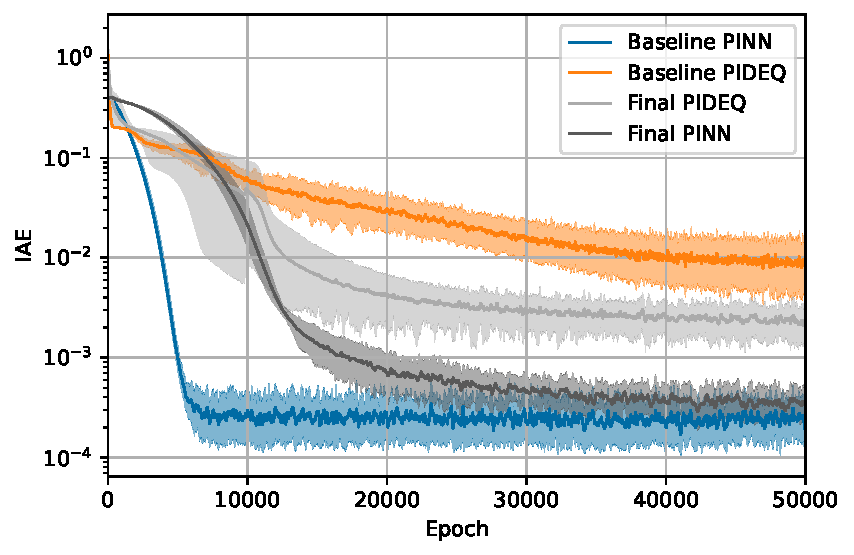
\includegraphics[width=.6\textwidth]{../images/final_iae.pdf}
	\caption{Learning curve of the final models and the baselines. ``Final PINN'', ``Final PIDEQ'' have 52 parameters.}
	\label{fig:final-iae}
    \end{figure}
\end{frame}

\begin{frame}
    % \frametitle{Final Model}
    \begin{figure}[h]
	\vspace{.1\textheight}
	\centering
	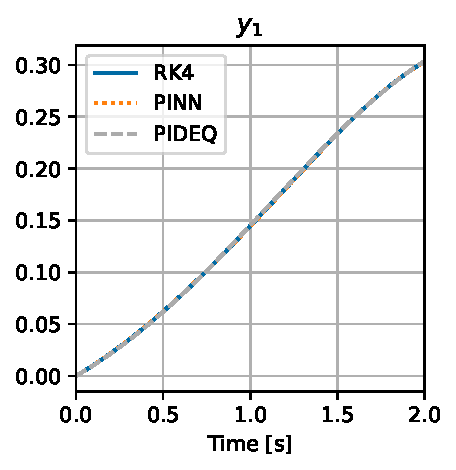
\includegraphics[width=.45\textwidth]{../images/final_vdp_y1.pdf}
	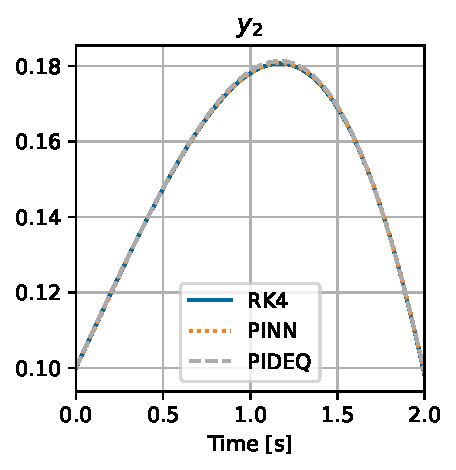
\includegraphics[width=.45\textwidth]{../images/final_vdp_y2.pdf}
	\caption{Prediction of PINN and PIDEQ in comparison to the reference approximation resulting from RK4.}
	\label{fig:final-vdp}
    \end{figure}
\end{frame}

\begin{frame}
    \frametitle{Van der Pol experiments}
    \begin{columns}[T] 
	\begin{column}{.6\textwidth}
	    \vspace{-10pt}
	    \begin{figure}[h]
	        \centering
		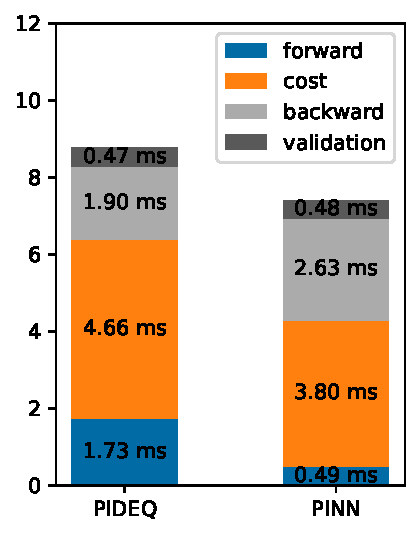
\includegraphics[width=.6\textwidth]{../images/final_times.pdf}
		\caption{Breakdown of median time per epoch for the final PIDEQ and PINN.}
		\label{fig:final-times}
	    \end{figure}
        \end{column}
	\begin{column}{.4\textwidth} 
	    \begin{description}
		\item[\textcolor{tabblue}{forward}] computing the output given the input during training;
		\item[\textcolor{taborange}{cost}] computing the cost function;
		\item[\textcolor{tabgray}{backward}] back-propagating the cost to the parameters;
		\item[\textcolor{tabdarkgray}{validation}] computing the output during validation (inference).
	    \end{description}
	\end{column}
    \end{columns}
    
\end{frame}

\begin{frame}
    \frametitle{Nonlinear Schrödinger experiments}
    Using the same approach, we compare a PIDEQ to the PINN trained by \cite{Raissi2019} for the NLS.

    \begin{figure}[h]
        \centering
	\begin{tikzpicture}
	    \node  (image) at (0,0) {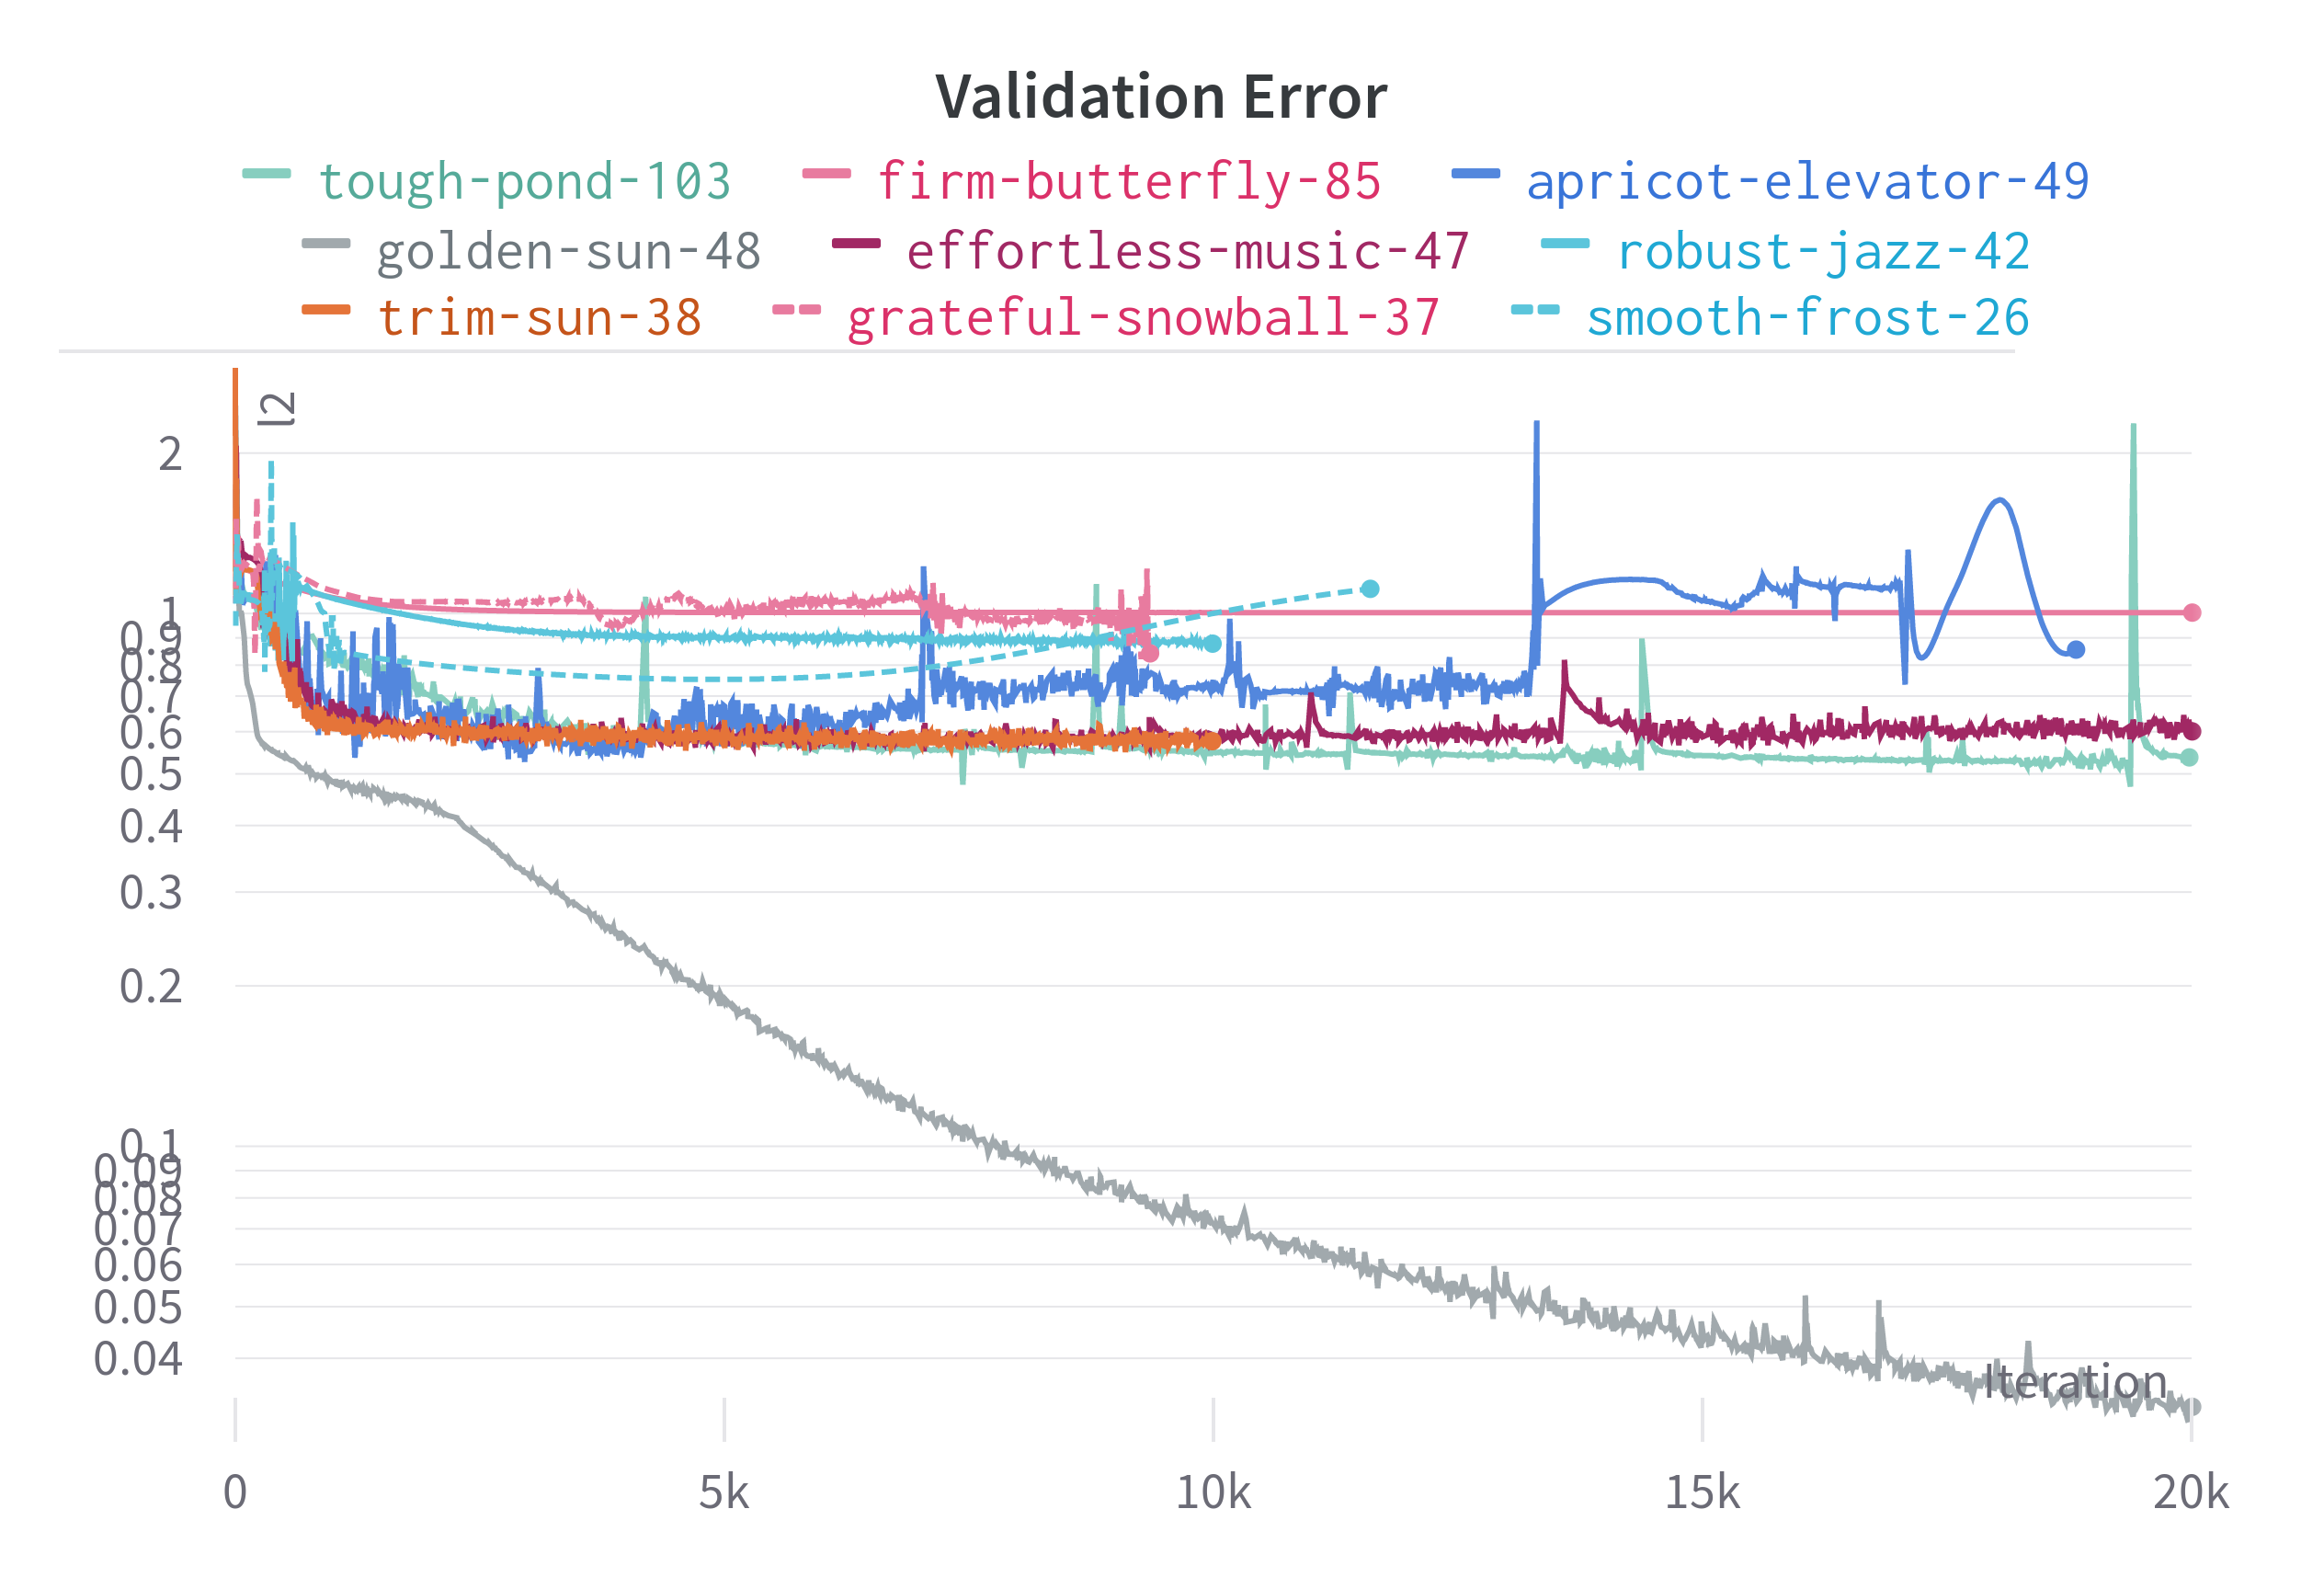
\includegraphics[width=0.6\textwidth]{nls-validation-ls.png}};
	    \node at (4,-1.7){PINN};
	    \node at (4.2,0.3){PIDEQs};
	\end{tikzpicture}
        \caption{Validation error ($l_2$) of PINN and PIDEQs solving NLS equations.}
        \label{fig:nls-validation-ls-png}
    \end{figure}
\end{frame}

\subsection{Regularization of DEQs}

\begin{frame}
    \frametitle{Regularization of DEQs}
    DEQs of the form \[
    \begin{cases}
	\bm{z} = \bm{f}_{\theta}\left( \bm{z},\bm{u} \right)  \\
	\bm{y} = C\bm{z} + D\bm{u}
    \end{cases}
    \] are unstable to train and do not provide any guarantees on the equilibrium.

    \begin{figure}[h]
        \centering
        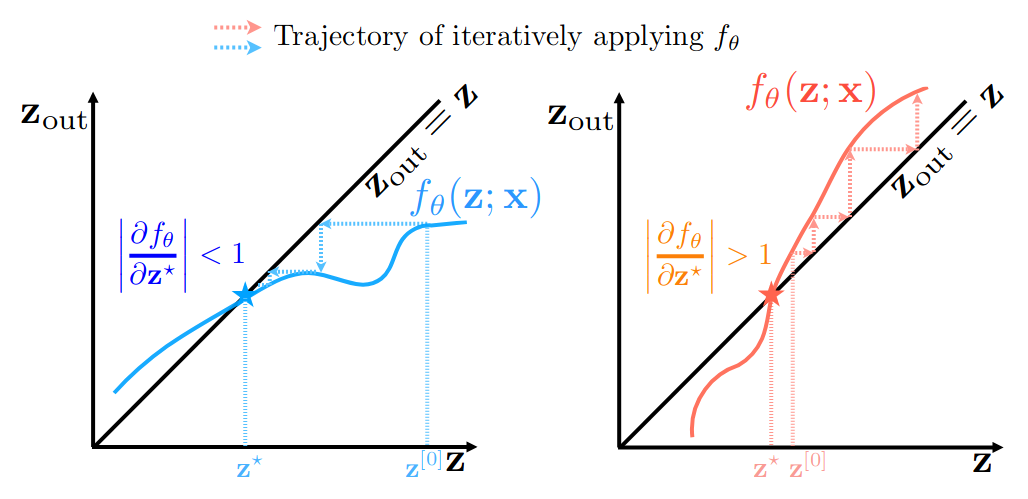
\includegraphics[width=0.6\textwidth]{reg-jac-f-theta.png}
        \caption{Examples of convergence and divergence of a DEQ on the iterative approach.}
        \label{fig:reg-jac-f-theta-png}
    \end{figure}
\end{frame}

\begin{frame}
    \frametitle{Regularization of DEQs}

    \begin{columns}
	\begin{column}{0.5\textwidth}
	    \cite{bai_stabilizing_2021}
	    \begin{itemize}[label={\textbullet}]
		\item Regularizes the spectral radius of $J_{\bm{f}_{\theta}}$;
		\item $\lambda_{PF}\left( J_{\bm{f}_{\theta}}\left( \bm{z}^{\star} \right)  \right) = \max\left( |\lambda_i| \right) \le \sqrt{tr\left( J_{\bm{f}_{\theta}}J_{\bm{f}_{\theta}}^T \right) } = \highlight{\|J_{\bm{f}_{\theta}}\|_{F}} $.
	    \end{itemize}
	\end{column}

        \begin{column}{0.5\textwidth}
	    \cite{Ghaoui2019}
	    \begin{itemize}[label={\textbullet}]
		\item $\bm{f}_{\theta} = \sigma\left( A\bm{z} + B\bm{u} \right)$;
	        \item $A$ is well-posed for $\sigma$ if the DEQ has a unique solution;
		\item $A\in WP\left( \sigma \right) \impliedby \lambda_{PF}\left( |A| \right) < 1  $;
		\item Enforces well-posedness through projected gradient descent on $1 > \highlight{\|A\|_{\infty}} \ge \lambda_{PF}\left( |A| \right)$.
	    \end{itemize}
        \end{column}
    \end{columns}
\end{frame}

\begin{frame}
    \frametitle{Regularization experiments}
    Different approaches on synthetic problem.

    \begin{figure}[h]
        \centering
        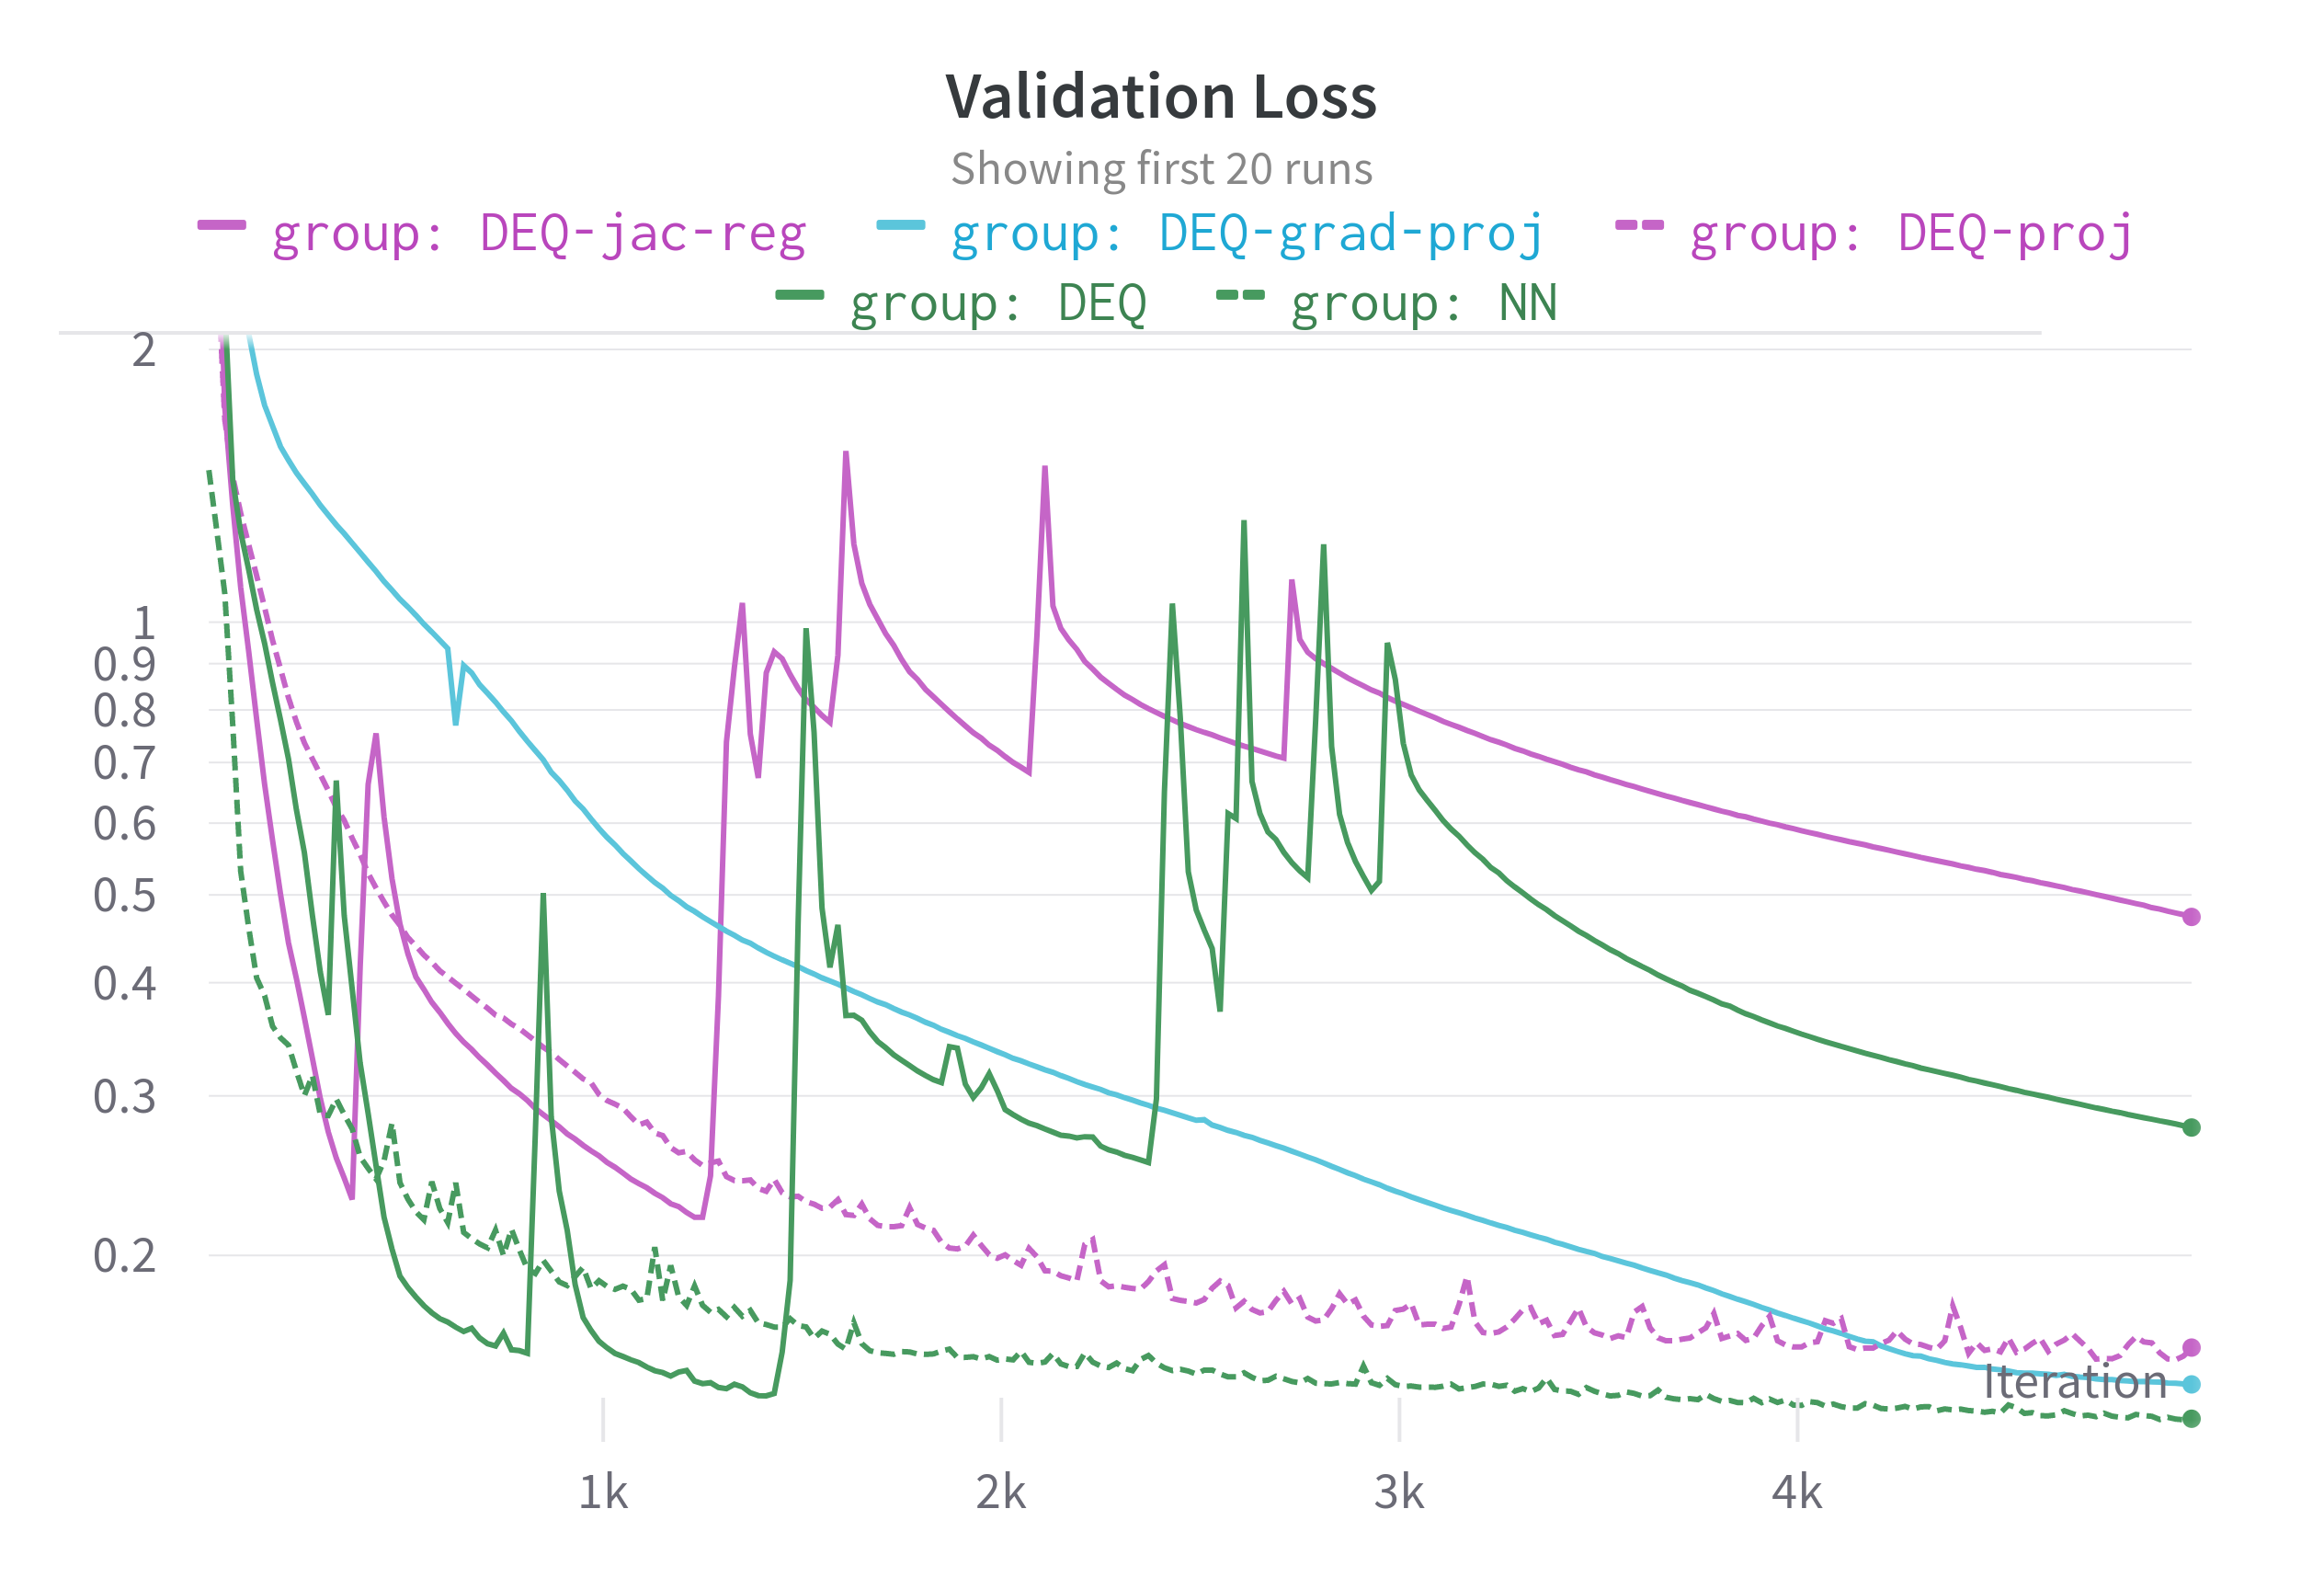
\includegraphics[width=0.6\textwidth]{dummy-val.png}
        \caption{Validation loss on synthetic dataset $y=5\cos\left( \pi u \right)\exp(-|u|/2)$.}
        \label{fig:dummy-val-png}
    \end{figure}
\end{frame}

\begin{frame}
    \frametitle{Regularization experiments}
    Different approaches on NLS.

    \begin{figure}[h]
        \centering
        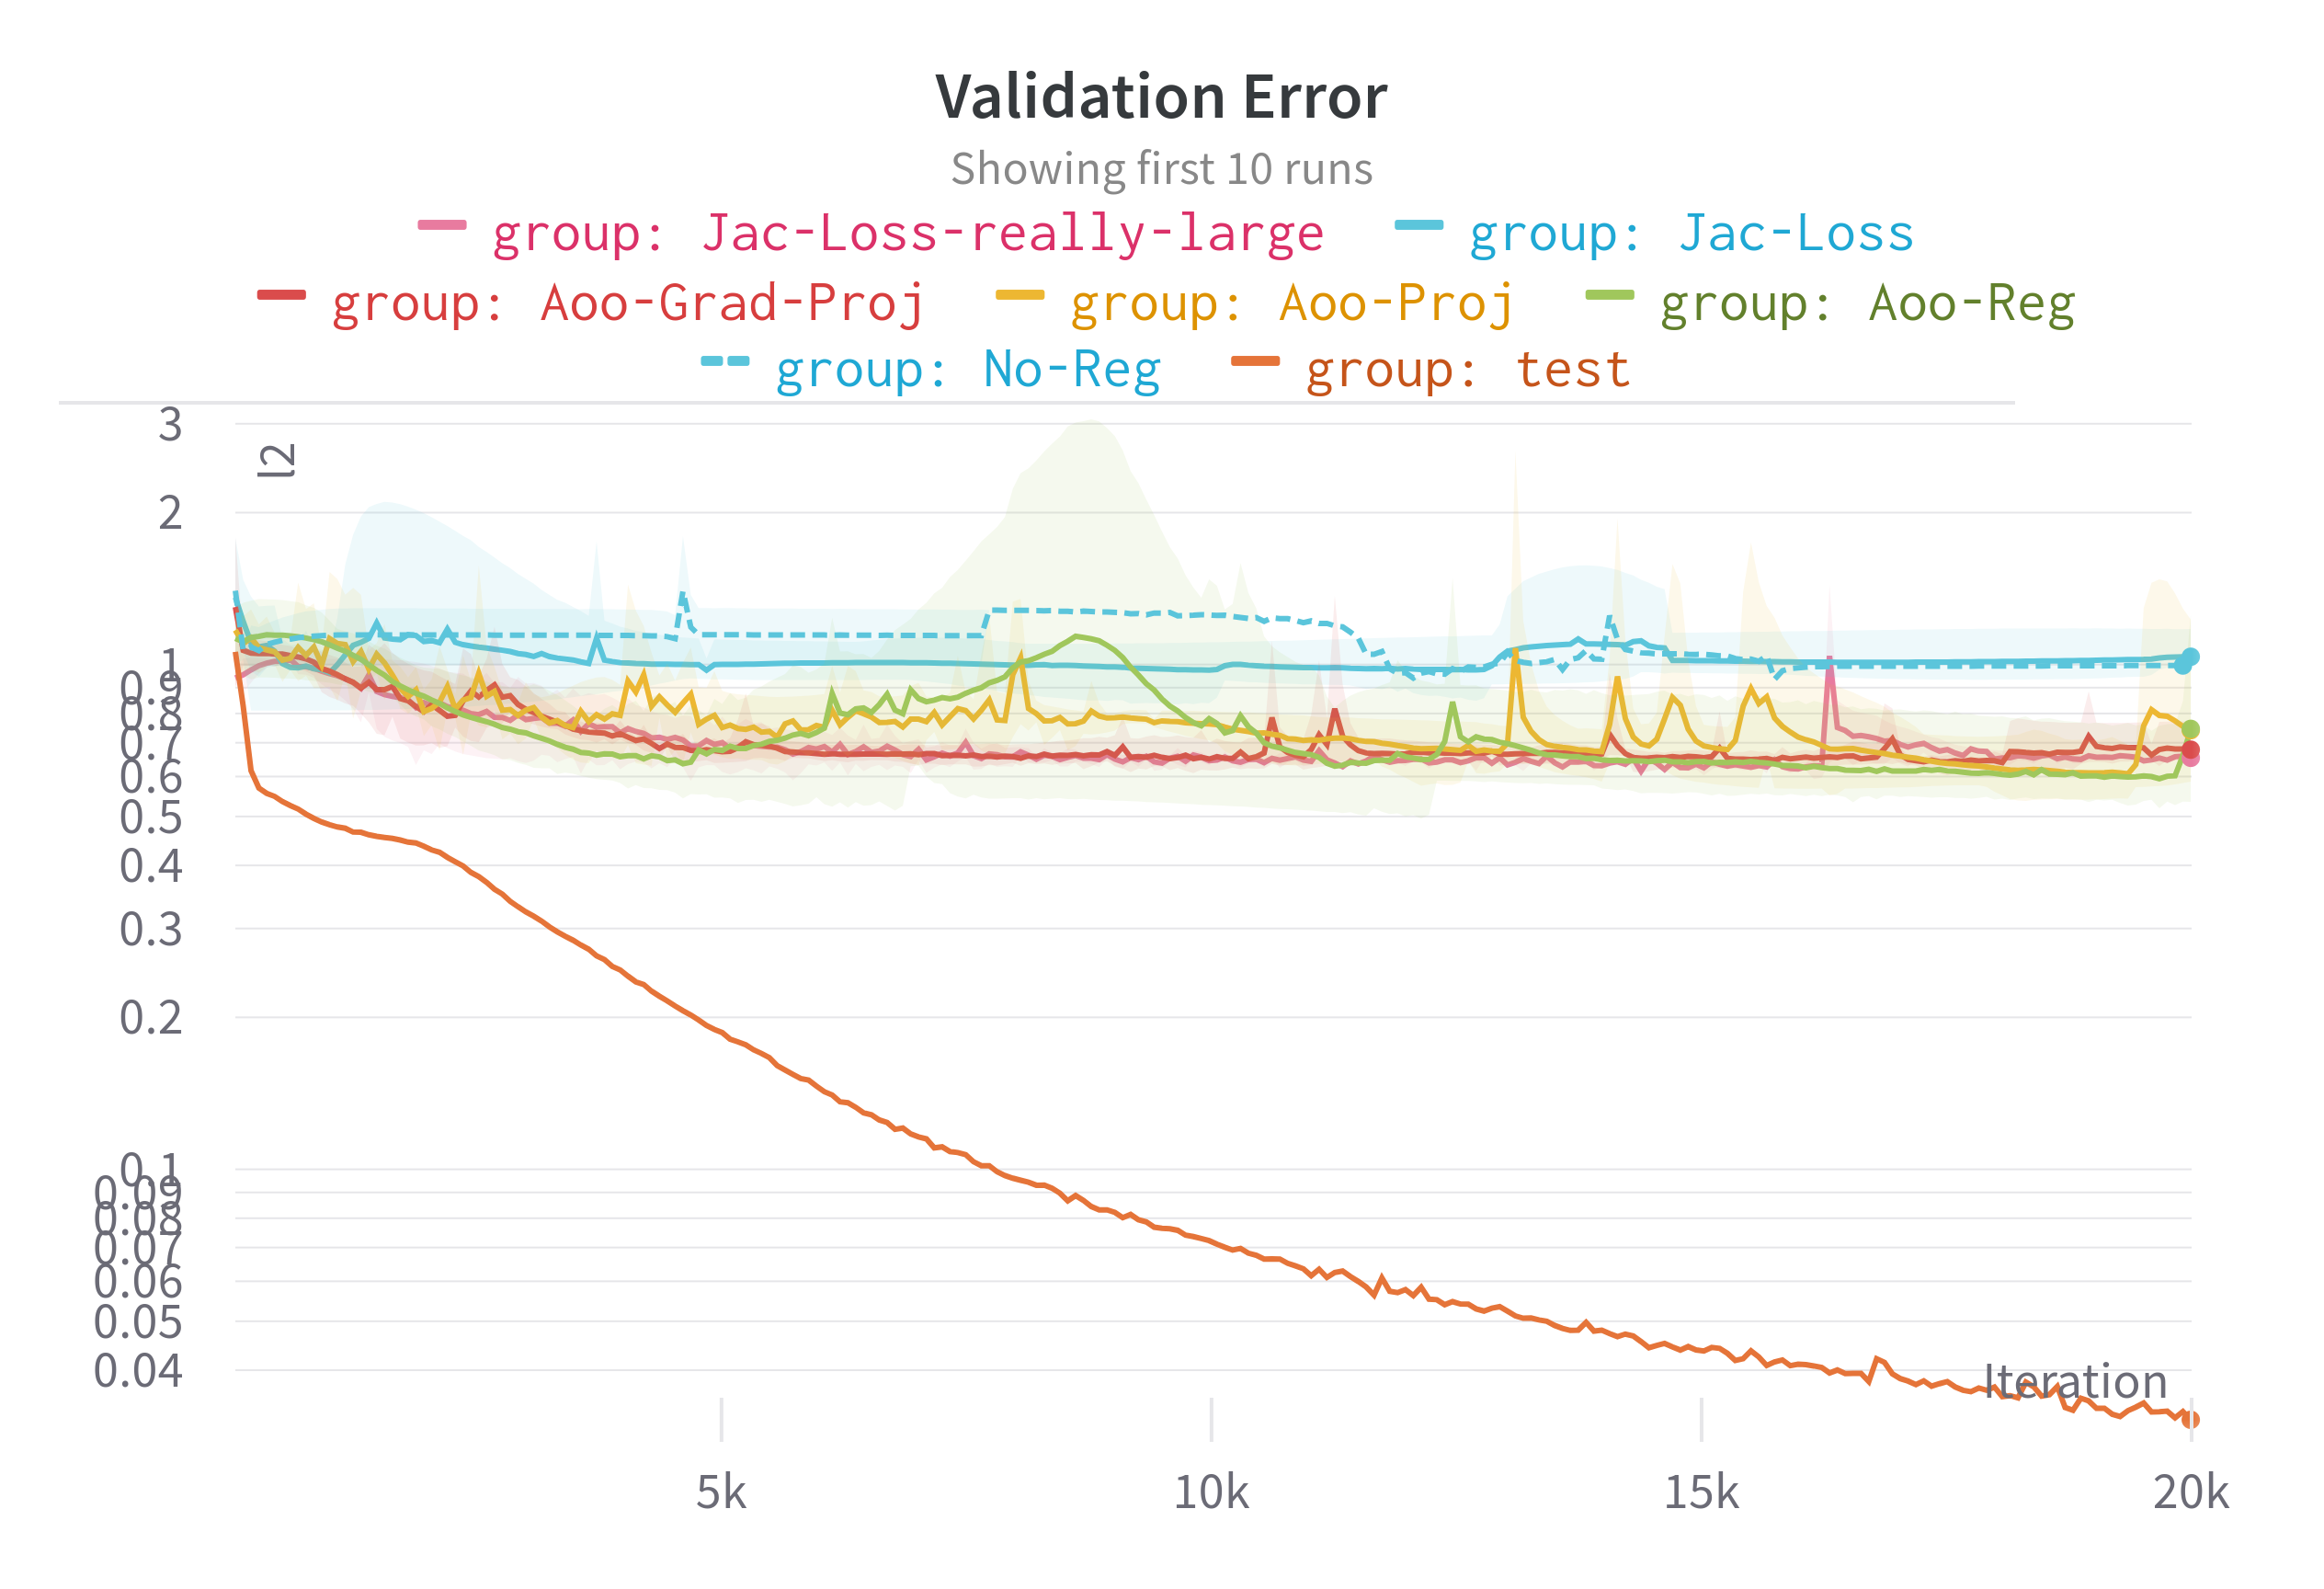
\includegraphics[width=0.6\textwidth]{nls_reg.png}
        \caption{Validation error on NLS.}
    \end{figure}
\end{frame}

\subsection{Higher-order Derivatives}

\begin{frame}
    \frametitle{Derivative of DEQs}
    Recap:
    Given a model
    \begin{align*}
	D^{EQ}_{\bm{\theta}}: \R^{n+1} &\longrightarrow \R^{m} \\
	\bm{x},t &\longmapsto 	D^{EQ}_{\bm{\theta}}(\bm{x},t) = \bm{z}^{\star} \\
	\bm{z}^{\star} &= f_{\bm{\theta}}\left( \bm{x},t, \bm{z}^{\star} \right)
    \end{align*}
    its derivative can be expressed \[
    \frac{d D^{EQ}_{\bm{\theta}}}{d (\cdot)}(\bm{x},t) = - \left[ \frac{d f_{\bm{\theta}}}{d \bm{z}}(\bm{x},t,D^{EQ}_{\bm{\theta}}(t)) - I \right]^{-1} \frac{d f_{\bm{\theta}}}{d (\cdot)}(\bm{x},t,D^{EQ}_{\bm{\theta}}(\bm{x},t))
    .\] 
\end{frame}

\begin{frame}
    \frametitle{Derivative of DEQs}
    As this inversion is impractical, the derivative is computed \[
	\frac{d D^{EQ}_{\bm{\theta}}}{d (\cdot)}(\bm{x},t) = - RootFind\left( \bm{v}^T\frac{d f_{\bm{\theta}}}{d \bm{z}} -\bm{v}^T - \bm{u}^T  \right)  \frac{d f_{\bm{\theta}}}{d (\cdot)}(\bm{x},t,D^{EQ}_{\bm{\theta}}(\bm{x},t))
    .\] \pause

    But any PIDEQ training requires (at least) second-order derivatives (Hessian) like $\frac{d^2 D^{EQ}_{\bm{\theta}}}{d t d (\cdot)}(\bm{x},t)$, which, through automatic differentiation, would imply in the \textcolor{red}{differentiation of $RootFind$} used in the backward pass. \pause
\end{frame}

\begin{frame}
    \frametitle{Derivative of DEQs}
    Our idea: Apply the implicit function theorem again and again to find analytical expressions for higher-order derivatives.
    \vfill

    This would speed up the training of PIDEQs on more complex applications (e.g., NLS).
\end{frame}

\section{Current Status}

\subsection{WIP}

\begin{frame}
    \frametitle{WIP}
    \vfill
    @ overleaf
    \vfill
\end{frame}


%%%
%%% Slide final
%%%
{
\usebackgroundtemplate{
\includegraphics[width=\paperwidth]{capa.png}}
\begin{frame}[plain,noframenumbering]
\vspace{15mm}
\begin{center}
\textcolor{cinza}{
\textbf{Thank you all}
}
\end{center}
\vspace{-6mm}
\begin{center}
\textcolor{cinza}{\scriptsize{
	Bruno M. Pacheco
}}
\end{center}
\vspace{-6mm}
\begin{center}
\textcolor{cinza}{\scriptsize{
mpacheco.bruno@gmail.com
}}
\end{center}
\vspace{-6mm}
\begin{center}
\textcolor{cinza}{\scriptsize{
\href{https://github.com/brunompacheco/pideq}{github.com/brunompacheco/pideq}
}}
\end{center}
\end{frame}
}

\begin{frame}[allowframebreaks,noframenumbering]
    \frametitle{References}
    \printbibliography
\end{frame}

\end{document}

